\documentclass[10pt, compress]{beamer}

\usetheme{m}

\usepackage{booktabs}
\usepackage[scale=2]{ccicons}
\usepackage{minted}

\usemintedstyle{trac}

\title{IT336 : Article Presentation}
\subtitle{Compiling a High-Level Language for GPUs (IBM)}
\date{\today}
\author{Alexandre Honorat}
\institute{Enseirb-Matmeca}

\begin{document}

\maketitle

\section{Introduction}

%\begin{frame}{Parallelism}
%    \begin{block}{Parallelism}
%        Execute several instructions at the same time on different data.
%    \end{block}
%    \begin{block}{Applications}
%        \begin{itemize}
%        \item image processing (SIMD)
%        \item scientific computation (often SIMD)
%        \item and \ldots ?
%        \end{itemize}
%    \end{block}
%    \begin{block}{Devices}
%        CPUs, GPUs, FPGAs
%    \end{block}
%\end{frame}


\begin{frame}{Article topic}
    \begin{block}{Easy programming : High-Level Language (HLL)}
        Authors introduce a new HLL language : \textbf{Lime}.\\
        \alert{Goal:} simple unique programming suitable for all different CPUs, GPUs, FPGAs
    \end{block}
    \begin{block}{Compilation}
        Automatized translation to a Low-Level Language.\\
        That is the difficult part \ldots
    \end{block}
\end{frame}

\begin{frame}{Related Work}
Several ways to write GPU parallelized code :
\begin{itemize}
\item HLL + Specific compiler 
    \begin{itemize}
    \item Lime + Lime
    \item StreamIt + Sponge
    \end{itemize}
\item API + specific device kernel code
    \begin{itemize}
    \item OpenCL, CUDA (only for NVIDIA chips)
    \end{itemize}
\item Framework/API + Runtime
    \begin{itemize}
    \item EXOCHI (for Intel chips), Quilin, StarPU, \ldots 
    \end{itemize}
\end{itemize}
\end{frame}

\section{Lime language}

\begin{frame}{Overview}
    \begin{block}{Oriented object .. and oriented stream language}
    Based on \textbf{Java}, with only a few more tokens.\\
    The output of a task is the input of the next one.
    \end{block}
    \begin{block}{How to express parallelism in the code}
        \begin{enumerate}
        \item write methods doing the computation, almost as in Java (except types)
        \item create tasks (calling your methods) and order it (to specify dependencies)
        \item call the tasks to be executed
        \item and finally, compile !
        \end{enumerate}
    \end{block}
\end{frame}

\begin{frame}{Syntax}
    \begin{block}{Types}
        \begin{itemize}
        \item \textbf{task}
        \item array, e. g. \textbf{float[ [ ] [ 4 ] ]}
        \end{itemize}
    \end{block}
    \begin{block}{Keywords}
    \hspace{4ex} \textbf{local} and \textbf{global} (for a function)
    \end{block}
    \begin{block}{Operators}
        \begin{itemize}
        \item \textbf{=>} : task flow operator
        \item \textbf{@} : map operator
        \item \textbf{!} : reduce operator
        \end{itemize}
    \end{block}
\end{frame}


\section{Lime compilation}

\begin{frame}{Neither a library nor a framework nor a compiler ...}
    You have to import \emph{lime.util.Tasks}, but lime is an \textbf{Eclipse Plugin} !
%    \pause
    \begin{block}{What code does Lime generate ?}
        \begin{itemize}
        \item \textbf{C} code
        \item \textbf{native} code (OpenCL, CUDA, \ldots)
        \item Java ByteCode or just Java ? or both ?
        \end{itemize}
    \end{block}
    \begin{block}{How is the code generated ?}
        Parsing method is not really explained.
        \alert{pattern matching} is used to recognize possible optimizations.
    \end{block}
\end{frame}

%\begin{frame}[fragile]
%\frametitle{How to generate good native code ?}
%    The main idea is to recognize task use of input/output data by pattern matching. 
%    \begin{exampleblock}{Local memory (OpenCL)}
%    \begin{minted}[fontsize=\small]{Java}
%    float[] doWork(float [] arg) {
%      ...
%      Parallel loop (i) {
%        float v = arg[i];
%        Parallel loop {
%          v;        
%        }
%      }
%      ...
%    \end{minted}
%    \end{exampleblock}
%\end{frame}

\begin{frame}{Internal working}
    \begin{figure}
    \centering
    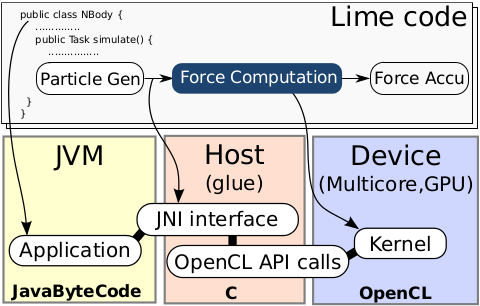
\includegraphics[scale=0.55]{images/lime_internal.png}
    \caption{Lime workflow}
    \label{img:lime_workflow}
    \end{figure}
\end{frame}


\begin{frame}{Data serialization}
    Lime have some own serializer to improve rapidity.
    \begin{figure}
    \centering
    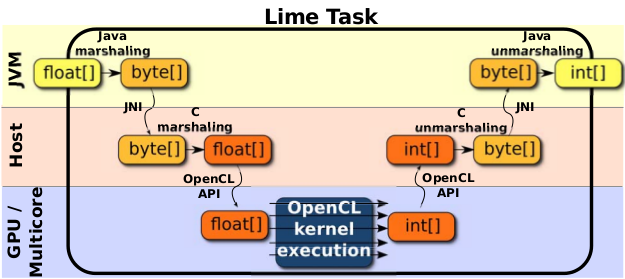
\includegraphics[scale=0.45]{images/lime_serialization.png}
    \caption{Lime serialization}
    \label{img:lime_serialization}
    \end{figure}
    \alert{Problem:} what about an array of tuples, and no specific serializer for this tuple ? Native serializer is too slow.
\end{frame}

\section{Benchmarks}

\begin{frame}{Methodology}
    \begin{block}{Tested algorithms}
    N-Body, Mosaic, some Parboil's benchmarks, \ldots
    \end{block}
    \begin{block}{Devices}
    CPU (Intel i7) and GPUs (some NVidia and AMD).
    \end{block}
    \begin{block}{Comparison}
        \begin{itemize}
        \item end-to-end speedup
        \item generated vs hand-tuned OpenCL
        \item communication time vs computation time
        \end{itemize}
    \end{block}
\end{frame}

\begin{frame}{Results}
    \begin{figure}
    \centering
    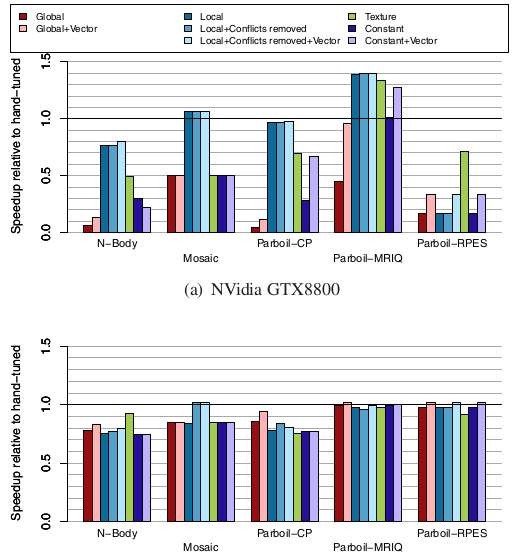
\includegraphics[scale=0.35]{images/lime_perf_hand.png}
    \caption{Lime performances compared to hand-tuned native code.}
    \label{img:lime_perf_hand}
    \end{figure}
\end{frame}

\section{Conclusion}

\begin{frame}{Pros and cons}
    \begin{exampleblock}{Pros}
    \begin{itemize}
    \item portability (Java and devices' abstraction)
    \item fast learning curve
    \item different way of programming (map reduce for tasks)
    \end{itemize}
    \end{exampleblock}
    \begin{alertblock}{Cons}
    \begin{itemize}
    \item does not compile without Eclipse Lime plugin
    \item Java
    \end{itemize}
    \end{alertblock}
\end{frame}

\plain{}{Personal conclusion}

\plain{}{Questions}

\end{document}
